%  PowerDomains.tex
%  Document created by seblovett on seblovett-NETBOOK
%  Date created: Wed 19 Feb 2014 11:26:11 GMT
%  <+Last Edited: Sun 16 Mar 2014 15:12:03 GMT by seblovett on seblovett-Ubuntu +>

\section{Power Techniques}
\subsection{Power Gating}

\subsubsection{Theory}

Power gating, in principle, is where the power to a module is switched off when not in use. 
By doing this, the module does not consume any power. 
It can be achieved by using either a header or a footer switch to disable either the supply connection or the ground connection. 
Figure \ref{fig:powerswitches} shows the realisation of the power gating circuits.

\begin{figure}[h]
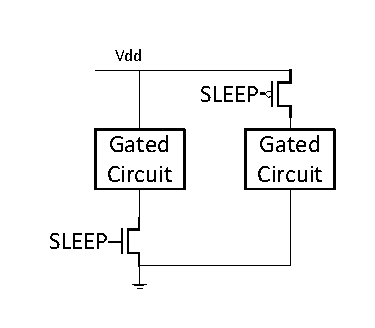
\includegraphics[width=0.5\textwidth]{Figures/powergating_switches.pdf}
\caption{Circuit diagrams showing the use of footer switches (left) or header switches (right).}
\label{fig:powerswitches}
\end{figure}

Although the theory of operation is simple, the technique poses many issues in the implementation.
Firstly, as the module is floating, the outputs are undefined.
This can cause the gates in another module to short circuit - at an input voltage of $ V_{dd} / 2 $, both the NMOS and PMOS transistors will be on, resulting in a direct line from supply to ground. 
The solution to this is is to add logic gates with a 'clamp' signal. 
This could be either an AND gate, of which the clamp signal is active low, or an OR gate with an active high clamp. 
This added logic is needed per signal output of the power gated module.

The second issue that power gating raises is when the gated module contains sequential logic. 
By removing the power to the sequential logic, the state is lost. 
This can then cause issues as state retention may be necessary, as well as low power.
The solution is to use a state retention register. 
There is a timing overhead involved to store the register before putting the device to sleep, disabling the majority of the circuit. 
State retention registers also require an individual power supply, meaning all power gated modules require two supplies; one which is gated and one constant supply.
A full realisation of a power gated circuit is shown in figure \ref{fig:powergated}. 


\begin{figure}
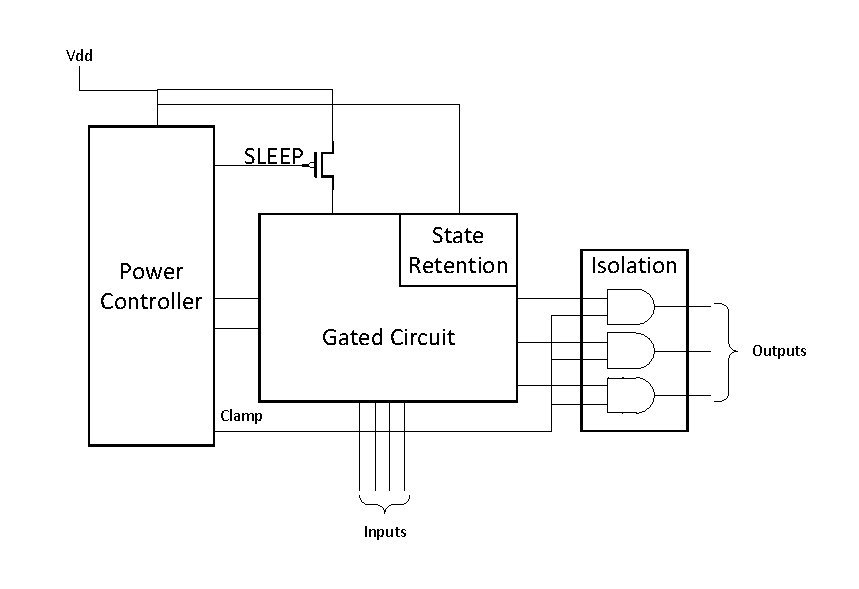
\includegraphics[width=0.5\textwidth]{Figures/powergating_full.pdf}
\caption{The relaisation of a power gated module. State retention, isolation and a power manager are all needed}
\label{fig:powergated}
\end{figure}


\subsection{Synthesis Techniques}




\subsection{Power Scaling}

%\inote{What actually am I wanting to discuss here?}
